\subsection{Herstellung mechanische Komponenten}
Die konzeptionellen CAD-Zeichnungen werden ab Semesterwoche 2 weiter 
ausgearbeitet, abgewickelt und die Fertigungszeichnungen erstellt. Hierbei 
müssen hauptsächlich Details wie Bohrungen für die Nieten angebracht und 
einige konstruktive Anpassungen vorgenommen werden. 

Ab Semesterwoche 3 können die ersten Teile an der Fräsmaschine im 
Elektrotechniklabor produziert werden, wobei parallel  hierzu die restlichen 
Komponenten am CAD fertiggestellt werden.  Um die gebogenen Innenkanten der 
Aussparungen zu realisieren, werden die gefrästen Blechteile mit einer 
Handpresse und eigens hierfür hergestellten Werkzeugen gefertigt.

In Semesterwoche 4 werden die Grundplatte zur Fertigung an der HSLU in Auftrag 
gegeben.

In Semesterwoche 5 werden zusätzlich einige Teile zum spanenden Herstellen, 
sowie zum 3D-Drucken in Auftrag gegeben. Ebenfalls wird eine 
Rohmaterialbestellung abgegeben.

Die in Auftrag gegebenen Teile können in Semesterwoche 6 abgeholt werden, 
wobei das  Rohmaterial fälschlicherweise aus Stahl, anstatt aus Aluminium, 
bestellt wurde. Eine neue Bestellung des richtigen Rohmaterials wurde abgesetzt.

In Semesterwoche 7 können die bestellten Teile sowie die zum biegen extern in 
Auftrag gegebenen Teile abgeholt werden. Des weiteren wird mit dem Zusammenbau 
der einzelnen Komponenten begonnen. Aufgrund eines beim Biegen entstandenen 
Verzugs einzelner Bauteile und einiger konstruktiver Ungenauigkeiten müssen 
diverse Bohrungen durch feilen nachgebessert werden. Durch Niethefter kann die 
Konstruktion bis zum endgültigen Vernieten aufgebaut werden.

\begin{figure}[h!]          
	\centering             
	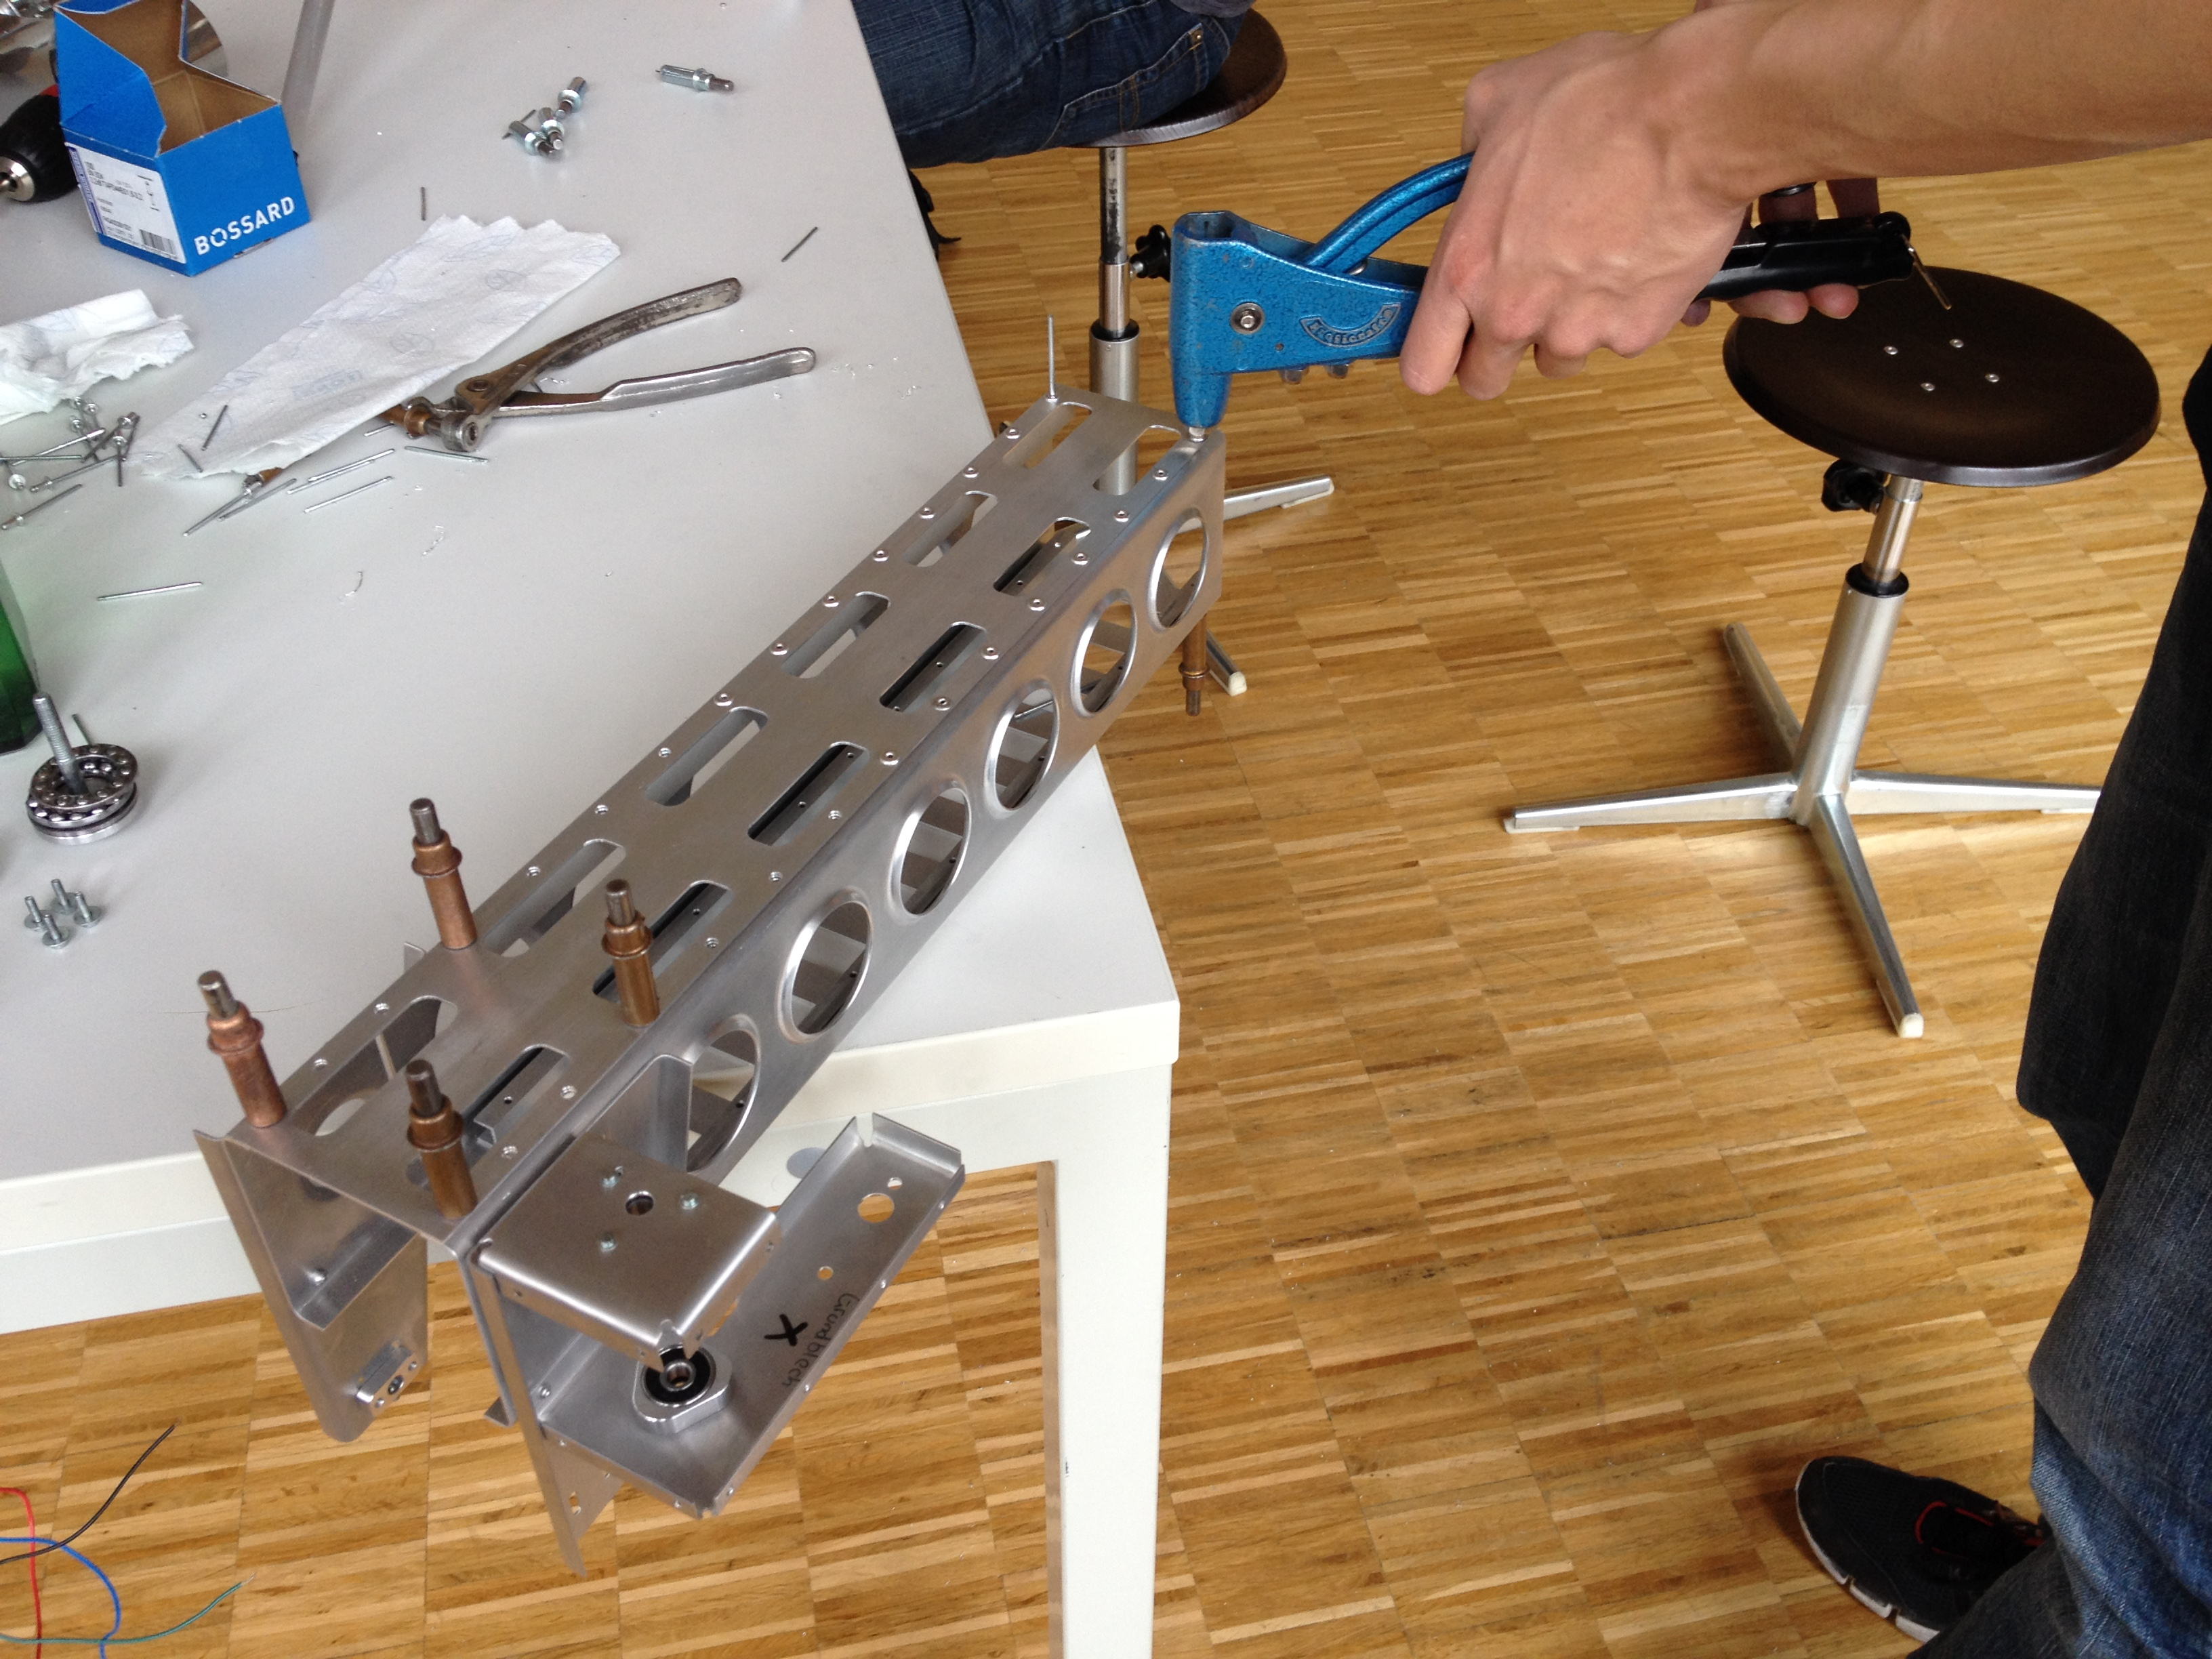
\includegraphics[width=0.5\textwidth]{fig/IMG_2290.JPG}
	\caption{Zusammenbau Balllager}
	\label{fig:Zusammenbau Balllager}        
\end{figure}

\begin{figure}[h!]          
	\centering             
	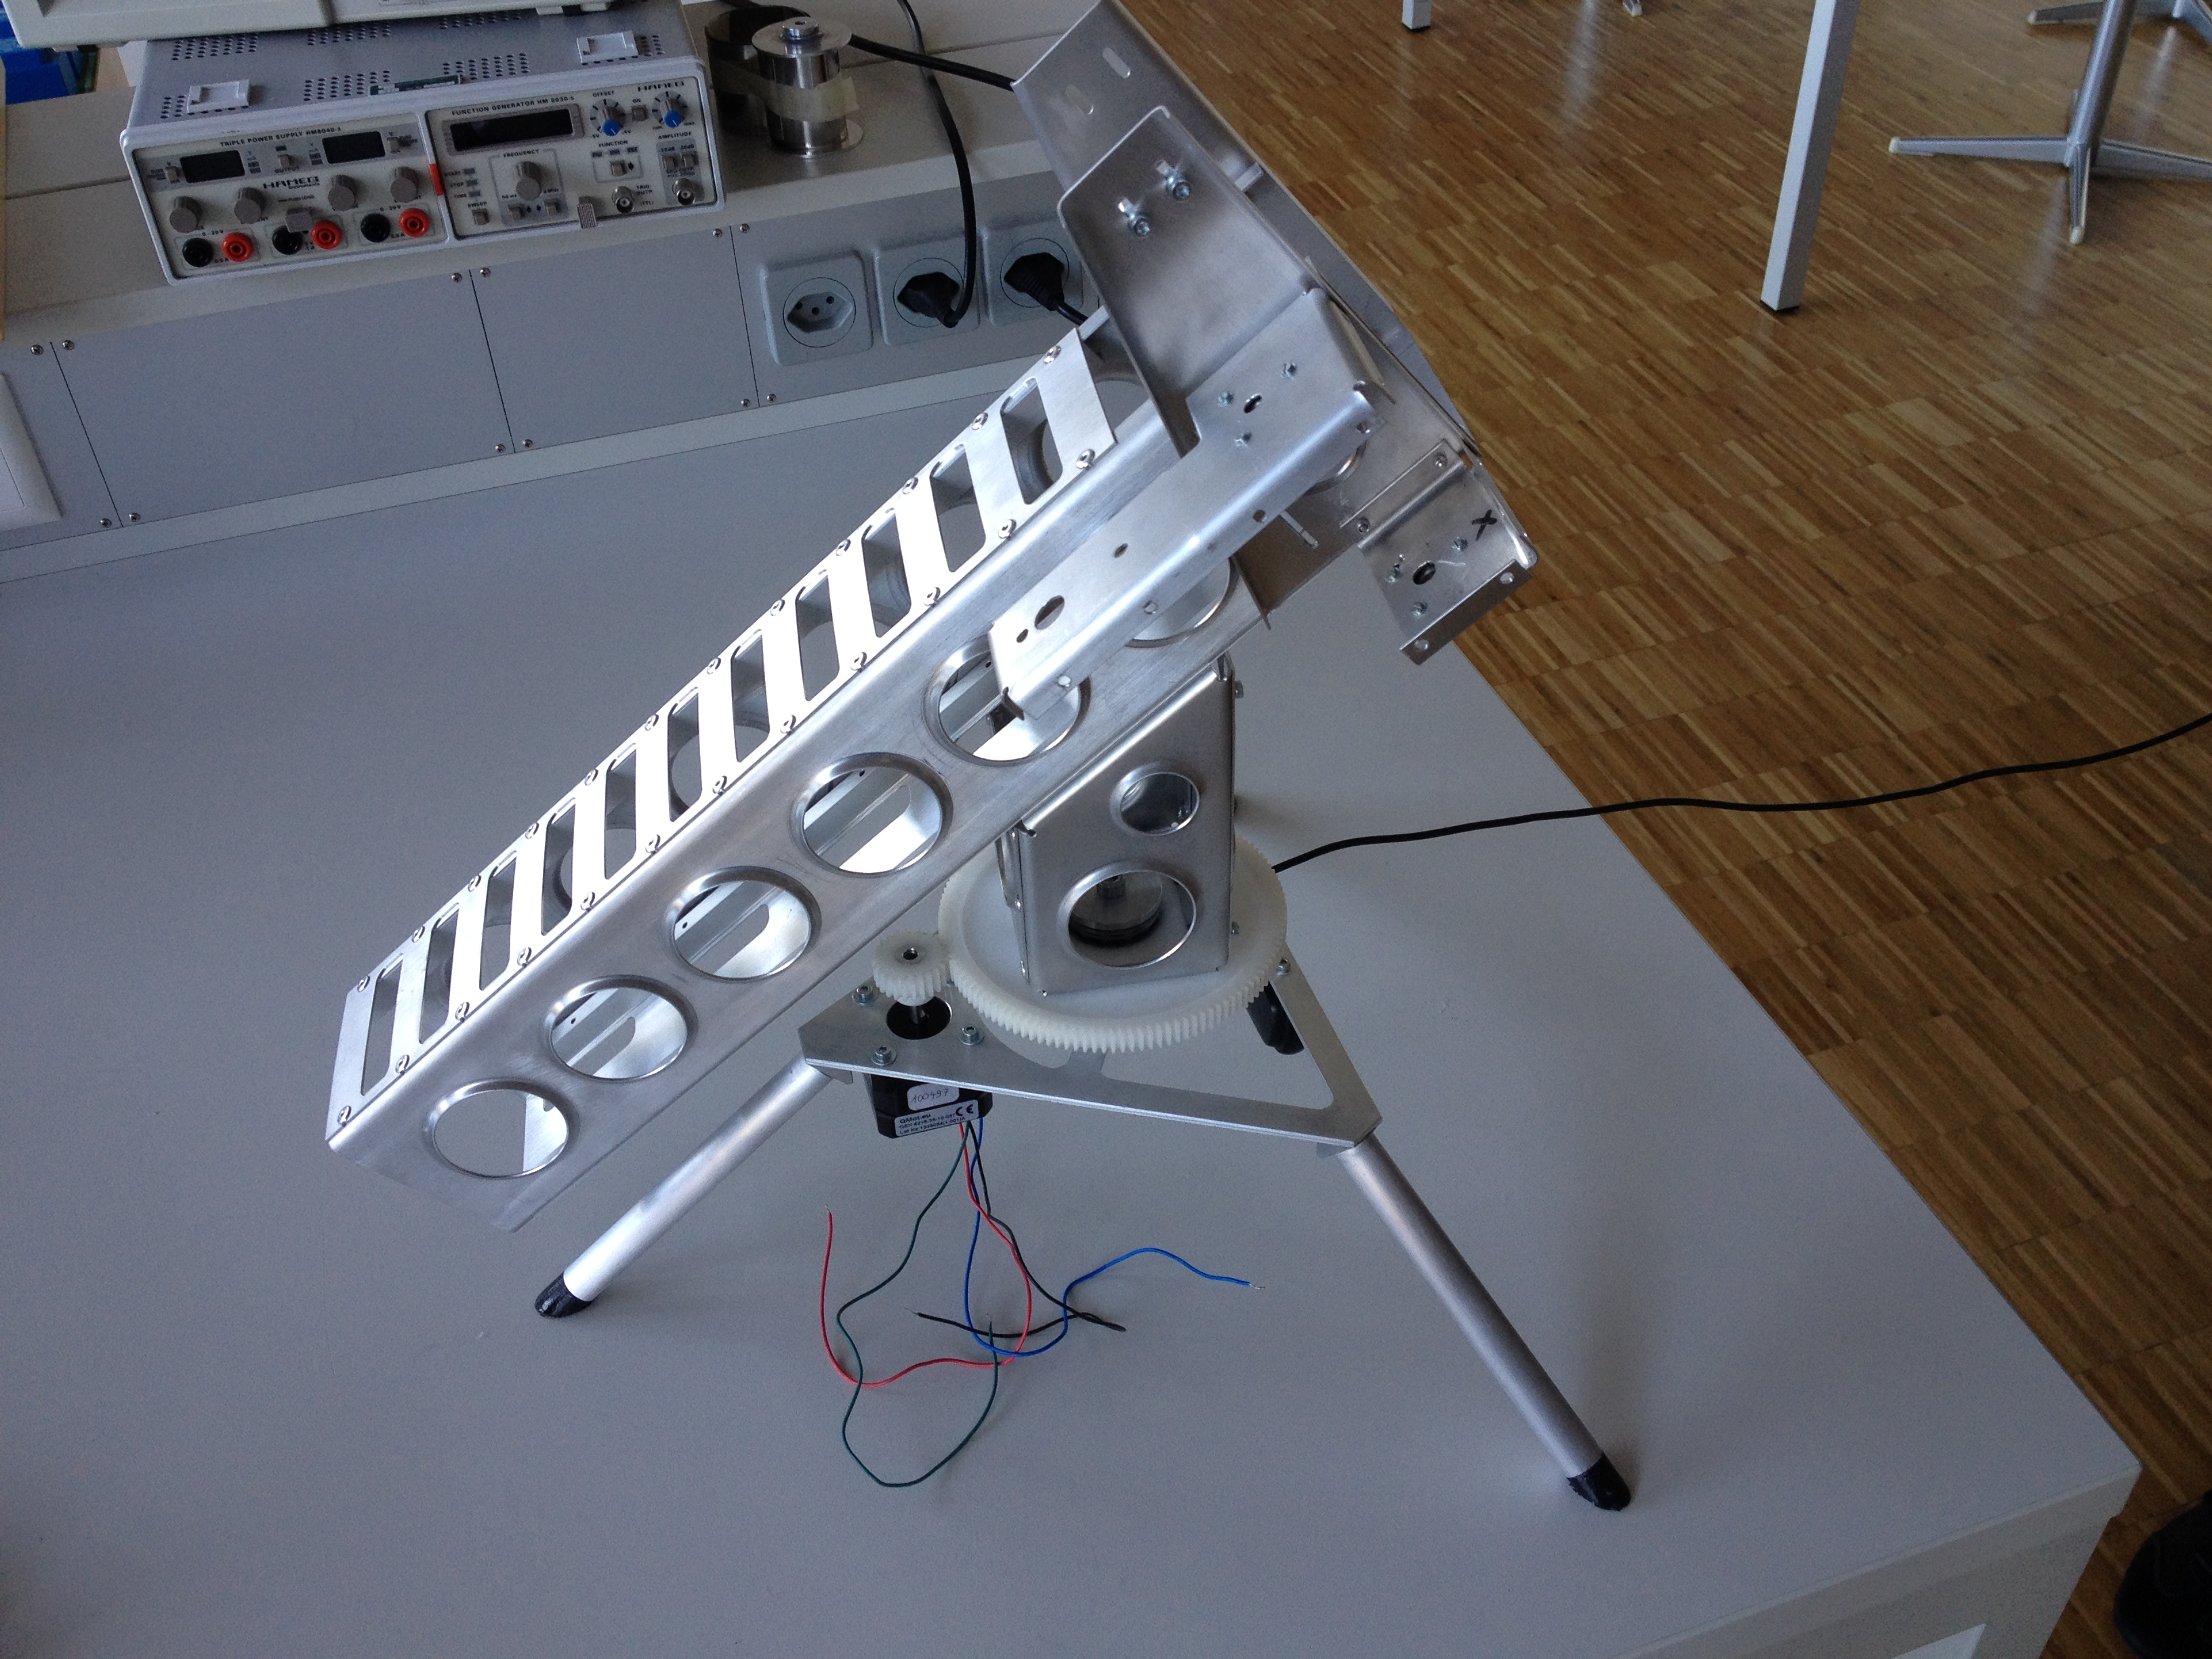
\includegraphics[width=0.5\textwidth]{fig/IMG_2303.JPG}
	\caption{Unvollständiger Aufbau}
	\label{fig:Unvollständiger Aufbau}        
\end{figure}

\paragraph{Nachfolgend werden die speziellen Anpassungen einzelner Komponenten genauer beschrieben:}

\paragraph{Balllager}
Anhand der Erfahrungen erster Testläufe wird entschieden, keine Verstärkung an 
der Unterseite des vorderen Endes anzubringen. Diese Verstärkung hätte eine zu 
starke Durchbiegung des Blechs beim Abschuss der Bälle verhindert.

\paragraph{Ballnachschub}
Beim Zusammenbau wird festgestellt, dass die Welle der Trommel einen zu 
grossen Durchmesser hat und daher mit Hilfe einer Handbohrmaschine und 
gewöhnlichem Schleifpapier auf das gewünschte Mass geschliffen werden muss.

\paragraph{Drehvorrichtung}
Um weiteres Gewicht einzusparen wird die bereits hergestellte Grundplatte auf die halbe Höhe überfräst.

\begin{figure}[h!]          
	\centering             
	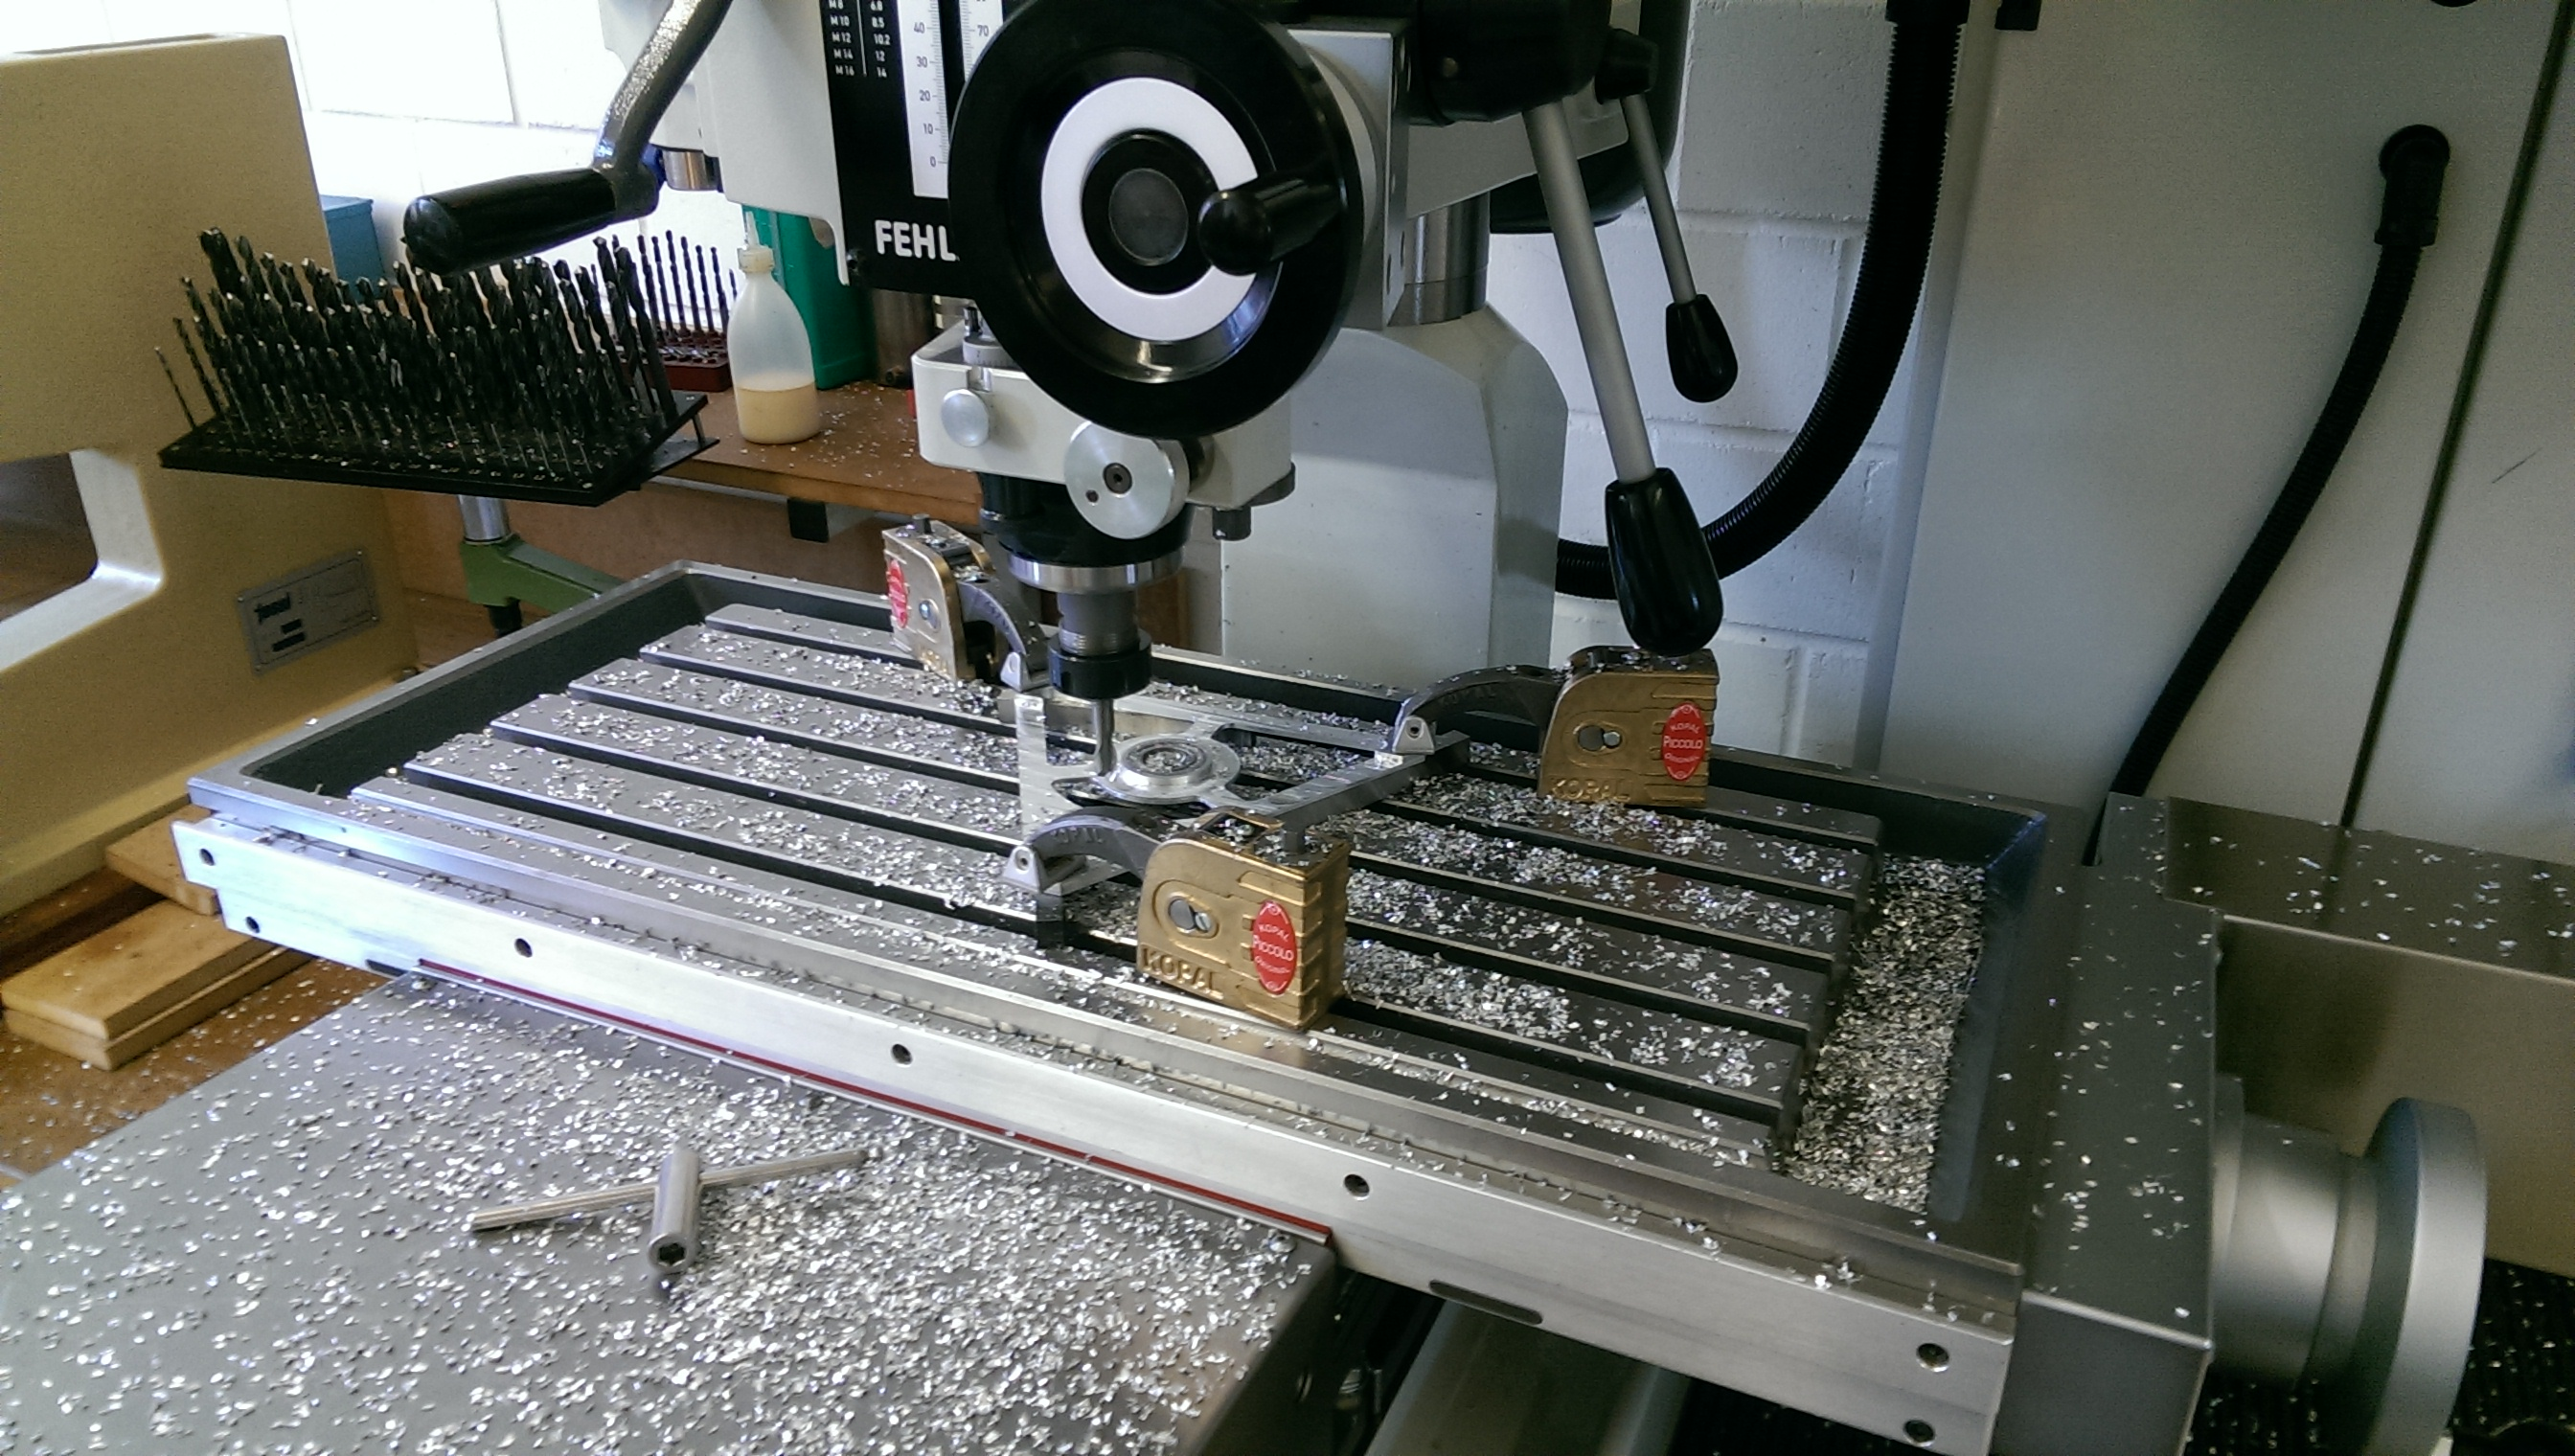
\includegraphics[width=0.5\textwidth]{fig/IMAG0357.jpg}
	\caption{Überfräsen der Grundplatte}
	\label{fig:Grundplatte fräsen}        
\end{figure}

\paragraph{Motor}
Sämtliche Magnete werden von Hand eingesetzt und mit Zweikomponentenklebstoff befestigt. Der Stator wird aus gebrauchten Floppydisk-Laufwerken ausgebaut, neu gewickelt, und an einer gefrästen Halterung befestigt.

Beim Zusammenbau wird bemerkt, dass die Langlöcher der Motorenhalterung zu kurz ausgeführt wurden um einen guten Anpressdruck der Bälle zu ermöglichen. Daher werden diese durch feilen verlängert.

\paragraph{Turm}
Die Muttern der Wartungsklappe werden auf der Innenseite des Turms mit Zweikomponentenklebstoff 
angebracht. 

\begin{figure}[h!]          
	\centering             
	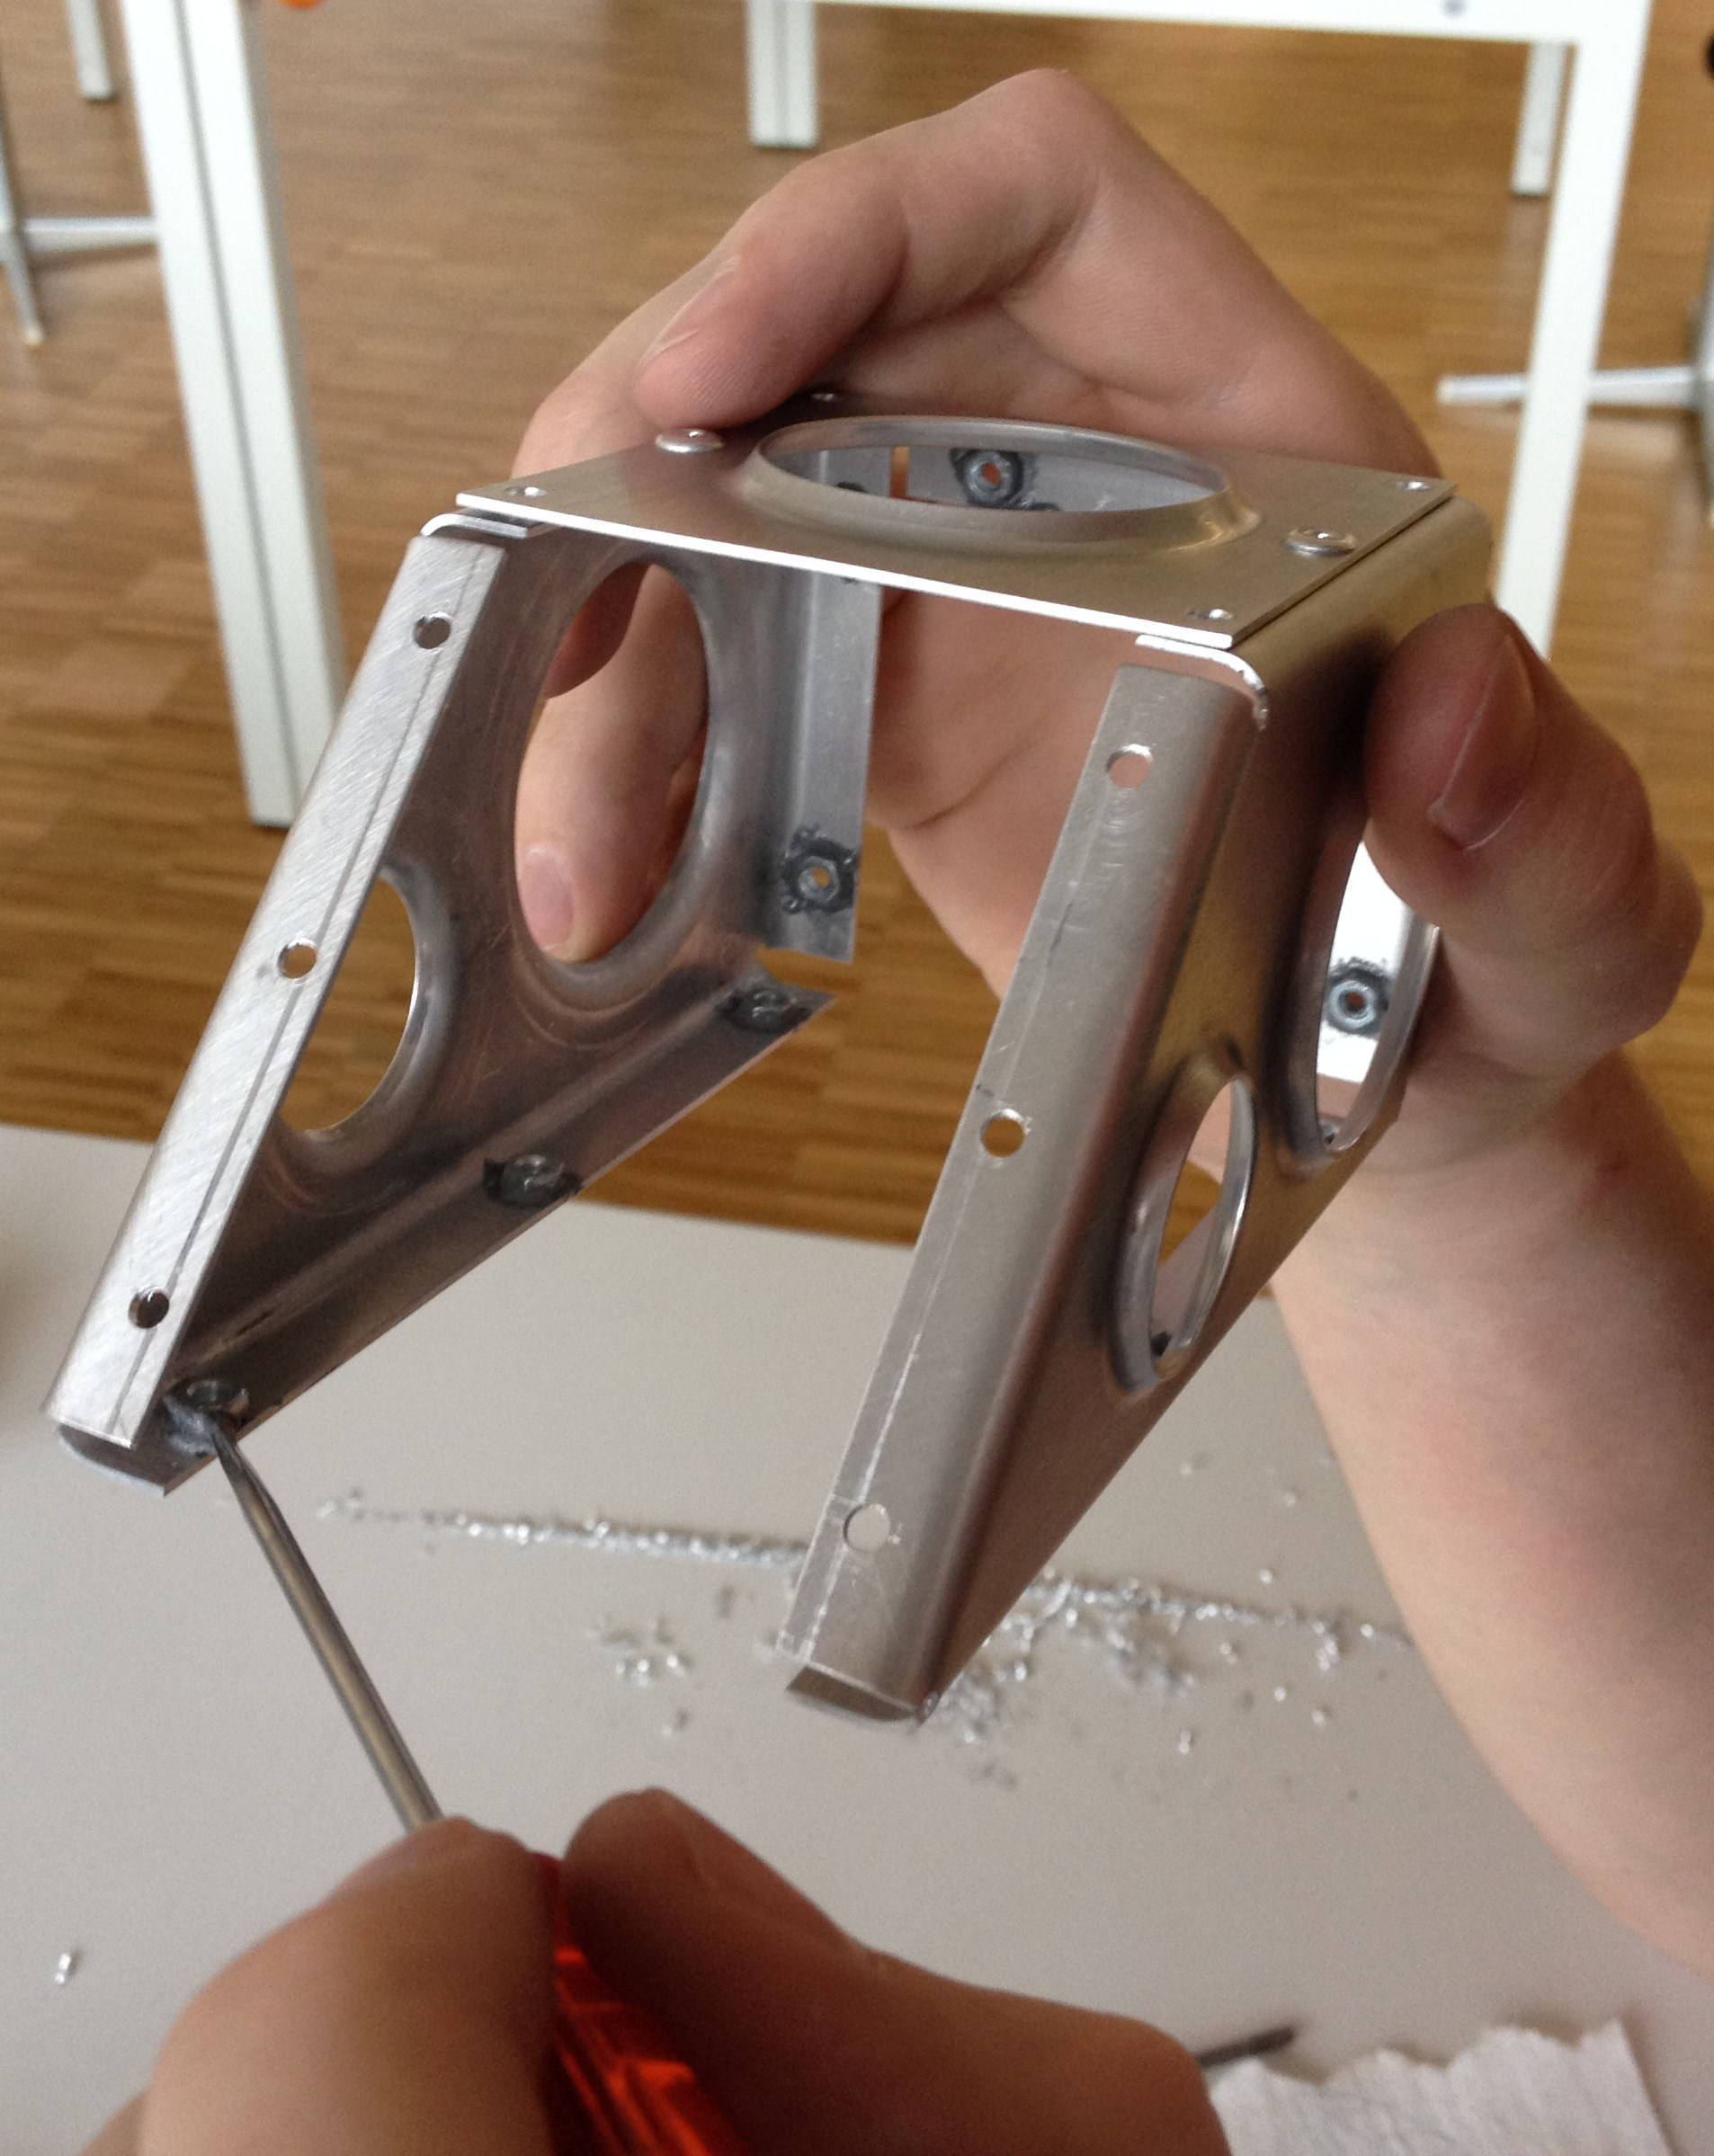
\includegraphics[width=0.3\textwidth]{fig/IMG_2292.JPG}
	\caption{Kleben der Muttern}
	\label{fig:Muttern Kleben}        
\end{figure}


